\documentclass[letterpaper,twocolumn,10pt]{article}

\usepackage{usenix}

%\usepackage[normalem]{ulem}

\usepackage{amsmath}
\usepackage{subfig}
\usepackage{booktabs}
%\usepackage{fullpage}
\usepackage{color}
\usepackage{xspace}
%\usepackage[hyphens]{url}
\usepackage{listings}
%\usepackage{comment}
\usepackage[hidelinks]{hyperref}
%\hypersetup{hidelinks}
%\usepackage[compact]{titlesec}
%\usepackage{pgf}

%\paperwidth=8.5in
%\paperheight=11in
%\setlength{\columnsep}{0.25in}
%\usepackage{leading}
%\usepackage[margin=1in]{geometry}

\usepackage{microtype}

%\titlespacing*{\section}{0pt}{0.5ex plus .1ex minus .1ex}{0ex}
%\titlespacing*{\subsection}{0pt}{0.5ex plus .1ex minus .1ex}{0ex}
%\titlespacing*{\subsubsection}{0pt}{0ex}{0ex}
%\titlespacing*{\paragraph}{0pt}{0ex}{5pt minus 3pt}

\frenchspacing
\renewcommand{\textfraction}{0.15}
\renewcommand{\floatpagefraction}{0.7}
\renewcommand{\dblfloatpagefraction}{0.7}

\setlength{\abovecaptionskip}{0.5em}
\setlength{\textfloatsep}{1em plus 0.2em minus 0.2em}

%\definecolor{xxxcolor}{rgb}{0.8,0,0}
%\iffalse
\newcommand{\XXX}[1]{}
%\else
%\newcommand{\XXX}[1] {{\color{xxxcolor} XXX: #1}\xspace}
%\fi

%%%
%%% Macros
%%%
% Instructions
\newcommand{\asm}[1]{\texttt{#1}}
% Code
\newcommand{\code}[1]{\texttt{\detokenize{#1}}}
% Command
\newcommand{\command}[1]{\texttt{\detokenize{#1}}}
% System Calls
\newcommand{\syscall}[1]{\texttt{\detokenize{#1}}}

%%%
%%% Code
%%%
\definecolor{lightgrey}{rgb}{0.95,0.95,0.95}

\lstdefinestyle{CSHStyle}{
    language=csh,
    basicstyle=\footnotesize\ttfamily,
    frame=tb,
    captionpos=b,
    columns=fullflexible,
    backgroundcolor=\color{lightgrey},
}

\lstdefinestyle{CStyle}{
    language=C,
    basicstyle=\footnotesize\ttfamily,
    frame=tb,
    captionpos=b,
    columns=fullflexible,
    backgroundcolor=\color{lightgrey},
}

\lstdefinelanguage[x64]{Assembler}
    [x86masm]{Assembler}
    {morekeywords={CDQE,CQO,CMPSQ,CMPXCHG16B,JRCXZ,LODSQ,MOVSXD,
		POPFQ,PUSHFQ,SCASQ,STOSQ,IRETQ,SWAPGS,MOVQ,
		ADDQ,SUBQ,MULQ,DIVQ,ANDQ,XORQ,INCQ,DECQ,
		CMPQ,CMPL,
		RDTSC,RDTSCP,
		XBEGIN,XEND,XABORT,XTEST,
		rax,rdx,rcx,rbx,rsi,rdi,rsp,rbp,
		r8,r8d,r8w,r8b,r9,r9d,r9w,r9b,
		r10,r10d,r10w,r10b,r11,r11d,r11w,r11b,
		r12,r12d,r12w,r12b,r13,r13d,r13w,r13b,
		r14,r14d,r14w,r14b,r15,r15d,r15w,r15b,
		xmm0,xmm1,xmm2,xmm3,xmm4,xmm5,xmm6,xmm7,
		xmm8,xmm9,xmm10,xmm11,xmm12,xmm13,xmm14,xmm15,
		ymm0,ymm1,ymm2,ymm3,ymm4,ymm5,ymm6,ymm7,
		ymm8,ymm9,ymm10,ymm11,ymm12,ymm13,ymm14,ymm15,
		zmm0,zmm1,zmm2,zmm3,zmm4,zmm5,zmm6,zmm7,
		zmm8,zmm9,zmm10,zmm11,zmm12,zmm13,zmm14,zmm15},
	morecomment=[l]\#
}

\lstdefinestyle{AsmStyle}{
    language=[x64]Assembler,
    basicstyle=\footnotesize\ttfamily,
    frame=tb,
    captionpos=b,
    belowskip=0.5em,
    columns=fullflexible,
    backgroundcolor=\color{lightgrey},
}




%\setcopyright{acmlicensed}

\begin{document}

\special{papersize=8.5in,11in}
\setlength{\pdfpageheight}{\paperheight}
\setlength{\pdfpagewidth}{\paperwidth}

\title{How Not To Build A Binary Translator}

\author{Aimilios Tsalapatis, Kenneth R Hancock}

\maketitle

Binary translation is a common method used to speed up the execution of
software components in systems that cannot run them natively.  The process
consists of dynamically creating native machine code corresponding to the
foreign binary.  While the concept is straightforward, there is a slew of ways
the construction of the translator can go awry, as will be outlined in this
paper.  We attempt to enumerate difficulties encountered while writing such an
assembler from the 6502 to the x86-64 architecture.  Examples include
dynamically rewriting the emitted code to connect basic code blocks, properly
allocating host registers to the guest code, and mixing emulation and binary
translation.  We discuss the nature of these problems, and offer advice for
anyone attempting to use this method.



\section{Introduction}

\subsection{Arguments for Binary Translation}

Binary Translation is the process through which a binary program meant for a
specific architecture can be run natively on another system.  Normally, binary
programs that cannot be run have to be interpreted instruction by instruction
with an emulator in order to reproduce its behavior.  However, this approach is
very slow, since the amount of native instructions executed for each foreign
one can be exceedingly high.

A way to speed up the execution of programs on arbitrary architectures is using
binary translation alongside emulation.  This technique takes advantage of the
fact that most architectures are composed of common commands, like moves and
rudimentary binary operations.  Therefore, it is possible to create native
executables that perform the same function as the original program.  The amount
of code needed run is lower, and execution is faster when compared to pure emulation.

Another use case for binary translation is software virtualization.  Some
programs need to access resources that are not accessible, because they do not
exist in the system.  Alternatively, the program does not have enough
privileges to modify the component, like in the case of userspace applications
attempting to change their page table register.

Virtual Machines (VMs) are such a class of programs.  The kernel running in the
VM is designed to have full access to the hardware, which in this case includes
sensitive processor registers and emulated devices.  A translator has the
responsibility of replacing code that attempts to do such accesses with
alternative instructions.  The program
emulates the resource in such a way that the VM can keep executing, and diverts
control back to it.  Popular emulators that employ binary translation, such as
Bochs and QEMU, utilize exactly this kind of scheme in order to emulate devices
like disks on demand.

\subsection{Binary Translation Internals}

Binary translation, much like all forms of compilation, hinges on the concept
of basic code blocks.  Basic blocks are sequences of machine instructions that
do not contain control flow commands like jumps and branches, and are the
smallest unit that binary translation works with.  More concisely, we can only
jump to the start of basic blocks. Programs are sectioned into multiple basic
blocks, which can be organized and viewed as a graph. Where nodes are the code
blocks themselves and directed edges represent a connection (through label or pointer)
from one code block to the other.  Nodes may have multiple edges to multiple nodes.

The concept of basic blocks is useful exactly because all programs enter the 
block from the beginning and exit from the end. That means that, as long as
the sum of its operations produce the same outputs for all possible inputs,
it is possible to transform the instructions without losing program correctness.
This is the fundamental principle behind compiler optimizations.

An emulator that employs binary translation goes through the program, creating and 
then executing a sequence of native instructions corresponding to the current block.
The key insight is that program correctness is independent of the underlying
platform, and is dependent only on creating the proper output for all inputs.
Therefore, it is possible to create a native program that does exactly that, using 
the original binary as a blueprint.





\begin{figure*}[ht] 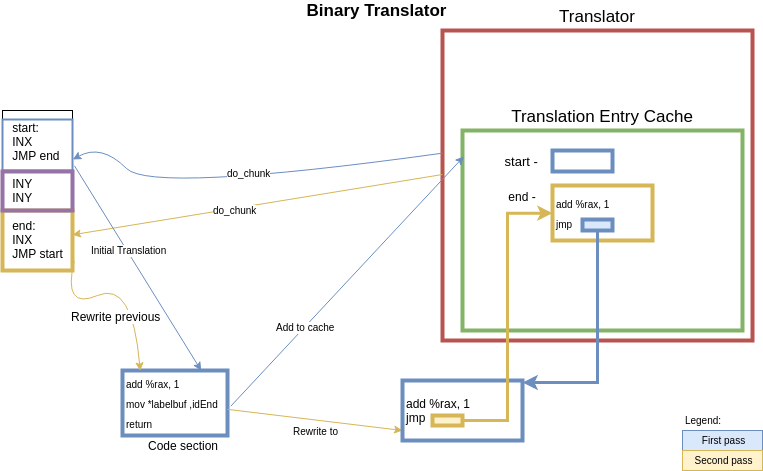
\includegraphics[width=\textwidth]{./images/translator.png}
\caption{The general overview of a simple binary translation} \label{fig:trans}
\end{figure*}

\section{A Better Design}

\subsection{Overview}

The general overview of a binary translator goes through the following steps.
And can be seen through Figure~\ref{fig:trans} 

\subsubsection{Retrieval} The translato reads until a jump or a label is found,
making note of every use of a label it encounters as it translates.  There are
two cases in which can occur at this point, either the end label  has been
encountered or it has not.  The easy case being if it has been encountered, in
which case we use a label cache and translate that instruction to jump to jump
to the code section pointed to by the cache.

If it has not, then we translate it such that when the assembly is executed it
moves a unique identifier for that label into a piece of shared memory and
returns.  This allows us so when we return from the assembly execution (which
may have been running through multiple different code sections), we know
exactly the label it requires, and also that it requires it immediately. We can
then scan the original binary for this label and start a new execution at that
label.

Code sections are just mapped pieces of memory that are executable.

\subsubsection{Edit} Once a basic code block has been fully translated, if the
block itself started with a label then it must notify and edit every block that
is currently in the request label map under said label. And retranslate those
blocks (we know there is possible optimizations for this, but for simplicity we
will just force a retranslate).

\subsubsection{Execute} Execution occurs through the bootstrapped assembly code
seen previously. Code sections are either executed seamlessly through each
other or upon exit we use unique identifier.





\section{Difficulties in Implementation}

For the implementation of the binary translator we opted to expand on our existing emulator project, written in C++.
The main idea was to have a translation cache in the emulator, which is queried for every basic block. 
If an existing translated block is found, then the emulator would instead execute that instead of going through the 6502 block instruction by instruction.

Creating executable code is straightforward, if somewhat awkward. First, an area of memory needs to be mmap()'ed as executable. 
The translator then emits instructions corresponding to the 6502 code by directly writing binary code into the buffer. 
Unfortunately, it is necessary to hardcode the opcodes in binary, since it is not possible to define code as data in C++. 
While it would in fact be simple to do so in pure x86 assembly, the fact that we are writing in a high level language actually makes the task more difficult.

x86\_64 assembly also has multiple versions of the same instruction, depending on the size and type of the operands that the opcode takes.
While the instruction set does succeed in its goal of being backwards compatible with as many past iterations of itself as possible, one disadvantage of this design choice is that there are a lot of opcodes that are obsolete for modern programs.
This one to many relation between instructions and opcodes means that a thorough understanding of the platform is necessary when deciding on a representation for a 6502 instruction.

A good example of the peculiarities of the x86 instruction set is the JMP instruction. 
This operation can execute either a near or a far jump, depending on the opcode used.
The differences between these two jumps are nonexistent in 64bit mode, since the distinction originates in the way the older members of the x86 family of processors implemented segmentation.
This method of partitioning memory has been rendered obsolete by virtual memory, however the opcodes are still there.

In order to find out which version of the instruction is actually the desirable one, we used a disassembler on compiled programs and inspected the opcodes corresponding to the JMP instructions used there.
This method turned out to be moderately useful: The disassembled code was always correct, however finding out the exact version of the instruction needed is not always guaranteed.
Looking for a perfect match instead of just a similar version was necessary because of the `polymorphism' that x86 instructions exhibit, which for example means that some instructions have different opcodes for 32-bit and 64-bit versions.

\begin{figure}[!h]
\begin{lstlisting}
    asm volatile (
        "pushq %%rax\n"
        "pushq %%rbx\n"
        "pushq %%rcx\n"
        "pushq %%rdx\n"
        "pushq %%r10\n"
        "xor %%rax, %%rax\n"
        "xor %%rbx, %%rbx\n"
        "xor %%rcx, %%rcx\n"
        "xor %%rdx, %%rdx\n"
        "xor %%r10, %%r10\n"
        "mov %[X], %%bl\n"
        "mov %[Y], %%cl\n"
        "mov %[A], %%dl\n"
        "callq *%[code]\n"
        "mov %%bl, %[X]\n"
        "mov %%cl, %[Y]\n"
        "mov %%dl, %[A]\n"
        "popq %%r10\n"
        "popq %%rdx\n"
        "popq %%rcx\n"
        "popq %%rbx\n"
        "popq %%rax\n"
        : [A] "+m" (A) , [X] "+m" (X), [Y] "+m" (Y) 
        : [code] "r" (code)
    );
\end{lstlisting}
	\caption {The inline assembly code used when entering and exiting the translated code.}
\end{figure}
 
A major problem we encountered was the linkage of the basic blocks into a self-contained x86 binary. 
As demonstrated in Figure \#, entering the emitted code is done by saving all registers to be used by the generated instructions.
As an optimization, the current values of the 6502 registers are always saved in specific registers for easy access.
Code generation is also simpler, since 6502 operations that act on the registers always get translated to x86 instructions that have a register as an operand.

The issues that came up have to do with the interplay of the binary translator with the emulator.
Normally, the emulator works at the instruction level, and does not need to be concerned with basic blocks.
This means that the existing infrastructure could not be used in combination with the binary translator without modifications:
Each time translated code is executed, the emulator is not capable of finding the next instruction that is supposed to be executed.

Monitoring the control flow of the generated code also proved to be a problem when connecting instructions together.
When connecting basic control blocks, the main idea is to overwrite the return function that has been attached at the end with a jump to the next block. 
This modification is especially complex with conditional branches. 
The basic blocks are disjoint in memory, since they have variable size and are created in a random order.
This means that the code for a relative branch looks like the following:

\begin{lstlisting}
	if (condition)
		jmp to taken
not taken:	
	jmp taken_path
taken:		
	jmp not_taken_path
\end{lstlisting}


%\bibliographystyle{abbrvnat}
%\bibliography{paper}

\end{document}


